\documentclass[11pt]{article}
\usepackage[utf8]{inputenc}

%%%%%%%%%%%%%%%%%%%%%%%%%%%%%%%%%%%%%%%%%%%%%%%%%%%%%%%%%%%%%%%%
% PACKAGES, FORMATTING, LISTING, AND OTHER GRAPHICAL ELEMENTS  %
%%%%%%%%%%%%%%%%%%%%%%%%%%%%%%%%%%%%%%%%%%%%%%%%%%%%%%%%%%%%%%%%

\usepackage{amsmath,amssymb}
\usepackage[T1]{fontenc} % font encoding
\usepackage{graphicx} % for figures
\usepackage{float} % for figures
\usepackage{indentfirst} % indent first paragraph of section
\usepackage{soul,xcolor} % for colors
\usepackage{xkcdcolors} % colors from XKCD color survey
\usepackage{mathtools} % for boxed equations within \align
\usepackage{sectsty} % adjust section headers
\usepackage{fancyhdr} % page headers
\usepackage{titling} % reference title,author,date (in fancyhdr page header)
\usepackage{breqn} % automatically line wrap long Eqs.
\usepackage{pdfpages} % for \includepdf
\usepackage{pdflscape} % landscape 
\usepackage{mdframed} % for framed environment
\usepackage{listings} % for code blocks
\usepackage{inconsolata} % better monospace font
\usepackage{matlab-prettifier} % Better MATLAB listing highlighting
\usepackage[letterpaper, total={6.5in, 9in}]{geometry} % set paper and margin size
\usepackage{empheq} % multiline boxed equations, etc.
\usepackage{hyperref}
\usepackage{dsfont}	% gives you \mathds{} font
% \usepackage{enumerate} % custom enumerate numbering (or lettering in this case)
\usepackage[shortlabels]{enumitem} % more enumerate options
\usepackage{svg} % use inkscape to import svgs
\usepackage{bm} % bold symbols
\usepackage[parfill]{parskip} % replace indentation with paragraph spacing
\usepackage{dsfont} % gives you \mathds{} font

% hyperbolic trig inverse functions
\DeclareMathOperator{\sech}{sech}
\DeclareMathOperator{\csch}{csch}
\DeclareMathOperator{\arcsec}{arcsec}
\DeclareMathOperator{\arccot}{arcCot}
\DeclareMathOperator{\arccsc}{arcCsc}
\DeclareMathOperator{\arccosh}{arcCosh}
\DeclareMathOperator{\arcsinh}{arcsinh}
\DeclareMathOperator{\arctanh}{arctanh}
\DeclareMathOperator{\arcsech}{arcsech}
\DeclareMathOperator{\arccsch}{arcCsch}
\DeclareMathOperator{\arccoth}{arcCoth} 

% add page headers
\pagestyle{fancy}
\fancyhf{}
\fancyhead[LE,LO]{\thetitle}
\fancyhead[RE,RO]{\theauthor}
\fancyfoot[CE,CO]{\thepage}

% adjust section header font size
\sectionfont{\fontsize{20}{15}\selectfont}
\subsectionfont{\fontsize{14}{15}\selectfont}

% vertical table spacing
\renewcommand{\arraystretch}{1.5}

% right-side cases
% \newenvironment{rcases}
%     {\left.\begin{aligned}}
%     {\end{aligned}\right\rbrace}

% Multi-line \fbox
\newcommand\multilineBox[1]{
\noindent
\fbox{
	\parbox{0.97\linewidth}
		{#1}
	}
}

% number just one equation in an un-numbered align* environment
\newcommand\numberthis{\addtocounter{equation}{1}\tag{\theequation}}

%%%%%%%%%%%%%%%%%%%%%%%%%%%%%%%%%%%%%%%%%%%%%%%%%%%%%%%%%%%%%%%%

% set listings font to inconsolata
\DeclareFixedFont{\ttb}{T1}{txtt}{bx}{n}{9} % for bold
\DeclareFixedFont{\ttm}{T1}{txtt}{m}{n}{9}  % for normal

% general listings environment
\lstnewenvironment{code}
{\lstset{
    frame=single,
    % backgroundcolor=\color{xkcdPale},
    basicstyle=\fontfamily{pcr}\selectfont\tiny
    }}
{}

% MATLAB listings environment
\lstnewenvironment{MATLAB}
{\lstset{
    style=Matlab-editor,
    frame=single,
    % backgroundcolor=\color{xkcdPale},
    basicstyle=\fontfamily{pcr}\selectfont\tiny
    }}
{}

% Python style for listings
\newcommand\pythonstyle{\lstset{
    language=Python,
    basicstyle=\ttm,
    morekeywords={self},              % Add keywords here
    keywordstyle=\ttb\color{xkcdGreen},
    morekeywords=[2]{
        array,
        pi,
        zeros,
        max,
        sin,
        cos,
        linspace,
        size,
        plot,
        xlabel,
        title,
        legend,
        show,
        concatenate,
        logspace,
        exp,
        ylabel,
        savefig,
        grid,
        figure,
        axes
    },
    keywordstyle = [2]{\color{xkcdBrightBlue}},
    emph={__init__},                  % Custom highlighting
    emphstyle=\ttb\color{xkcdRed},    % Custom highlighting style
    stringstyle=\color{xkcdGreen},
    backgroundcolor=\color{xkcdPale},
    numberstyle=\color{xkcdGrey},
}}

% Python listings environment
\lstnewenvironment{python}[1][]
{\pythonstyle \lstset{#1}}
{}

% Python listings for external files
\newcommand\pythonexternal[2][]
{{\pythonstyle \lstinputlisting[#1]{#2}}}

% Python listings inline
\newcommand\pythoninline[1]{{\pythonstyle \lstinline!#1!}}


%%%%%%%%%%%%%%%%%%%%%%%%%%%%%%%%%%%%%%%%%%%%%%%%%%%%%%%%%%%%%%%%
% MATHEMATICAL SHORTCUTS                                       %
%%%%%%%%%%%%%%%%%%%%%%%%%%%%%%%%%%%%%%%%%%%%%%%%%%%%%%%%%%%%%%%%

% real and imaginary components
\renewcommand{\Re}{\operatorname{Re}}
\renewcommand{\Im}{\operatorname{Im}}

% Fourier transforms
\newcommand\fourier[1]{\frac{1}{\sqrt{2\pi}} \int_{-\infty}^\infty #1 e^{-i\omega x} \textrm{d}x}
\newcommand\inverseFourier[1]{\frac{1}{\sqrt{2\pi}} \int_{-\infty}^\infty #1 e^{i\omega x} \textrm{d}\omega}

% derivatives
\newcommand{\ppf}[2]{\frac{\partial #1}{\partial #2}}
\newcommand{\pppf}[3]{\frac{\partial^2 #1}{\partial #2 \partial #3}}
\newcommand{\ddf}[2]{\frac{\text{d} #1}{\text{d} #2}}
\newcommand{\DDf}[2]{\frac{\text{D} #1}{\text{D} #2}}

% norms
\newcommand\norm[1]{\lVert#1\rVert}

% statistical operators
\newcommand{\prob}{\operatorname{P}}
\newcommand{\expectation}{\operatorname{E}}
\newcommand{\variance}{\operatorname{Var}}
\newcommand{\stddev}{\operatorname{SD}}

% statistical distributions
\newcommand{\bernoulli}{\operatorname{Bernoulli}}
\newcommand{\binomial}{\operatorname{Binomial}}
\newcommand{\poisson}{\operatorname{Poisson}}
\newcommand{\normal}{\operatorname{Normal}}

%%%%%%%%%%%%%%%%%%%%%%%%%%%%%%%%%%%%%%%%%%%%%%%%%%%%%%%%%%%%%%%%
% COMMONLY USED COPYPASTAS
%%%%%%%%%%%%%%%%%%%%%%%%%%%%%%%%%%%%%%%%%%%%%%%%%%%%%%%%%%%%%%%%

% CODE BLOCK

% \begin{MATLAB}[caption={MATLAB script},label={code:p1}]
% for i = 1:n
%     disp('string')
% end
% \end{MATLAB}
% Code block \ref{code:p1}



% MULTIPLE EQUATIONS BOXED

% \begin{empheq}[box=\fbox]{align}
% \end{empheq}



% ENUMERTATE WITH a) instead of 1.

% \begin{enumerate}[label=\alph*)]
% \end{enumerate}
% 'Problem' sections
% \renewcommand{\thesection}{Part \arabic{section}}
\renewcommand{\thesubsection}{\arabic{section}.\alph{subsection}}
% \renewcommand{\thesubsection}{\arabic{subsection}}

\title{ENGR 510 Signals Homework}
\author{Anthony Su}
\date{December 6, 2024}

\begin{document}
\thispagestyle{plain}
\maketitle


%%%%%%%%%%%%%%%%%%%%%%%%%%%%%%%%%%%%%%%%%%%%%%%%%%%%%%%%%%%%%%%%%%%%%%%%%%%%%%%%
% 1. Building an Orthogonal Cosine Basis
%%%%%%%%%%%%%%%%%%%%%%%%%%%%%%%%%%%%%%%%%%%%%%%%%%%%%%%%%%%%%%%%%%%%%%%%%%%%%%%%
\section{Building an Orthogonal Cosine Basis}

\subsection{} % a --------------------------------------------------------------
Let $f(x) = \cos(\pi m x)$ and let $g(x) = \cos(\pi n x)$ where $m \neq n$ and
$m, n \in \mathbb{Z}$.
Then, on the interval $[0, 1]$,
\begin{align*}
    \langle f, g \rangle &= \int_0^1 f(x) g(x) \mathrm{d}x \\
    \langle f, g \rangle &= \int_0^1 \cos(\pi m x) \cos(\pi n x) \mathrm{d}x \\
    \langle f, g \rangle &= \left.\frac{1}{2 \pi}\left(
        \frac{\sin(\pi x (m-n))}{m-n} + \frac{\sin(\pi x (m+n))}{m+n}
        \right)\right|_0^1 \\
    \langle f, g \rangle &= \frac{1}{2 \pi}\left(
        \frac{\sin(\pi (m-n))}{m-n} + \frac{\sin(\pi (m+n))}{m+n}
        - \frac{\sin(0)}{m-n} - \frac{\sin(0)}{m+n}
        \right)
\end{align*}
Since $m$ and $n$ are integers, $\sin(\pi (m \pm n))=0$. Simplifying,
\begin{align*}
    \langle f, g \rangle &= 0
\end{align*}
\begin{mdframed}
    Thus, $\cos(\pi m x)$ and $\cos(\pi n x)$ are orthogonal for $m \neq n$ and
    $m, n \in \mathbb{Z}$.
\end{mdframed}

\subsection{} % b --------------------------------------------------------------
\begin{listing}[H]
    \caption{Python code to generate Figure \ref{1bfig1}}
    \label{1blst1}
    \begin{minted}{python}
        x_vec = np.arange(0, 1.01, 0.01)
        fig, ax = plt.subplots(figsize=(5, 2.5), layout='constrained')
        for m in range(6):
            y_vec = np.cos(np.pi * m * x_vec)
            ax.plot(x_vec, y_vec, label=f'm={m}')
        ax.set_xlabel('x')
        ax.set_ylabel('f(x)')
        ax.legend()
        ax.grid(True)
        fig.savefig('1bfig1.png', dpi=300)
        plt.show()
    \end{minted}
\end{listing}
\begin{figure}[H]
    \centering
    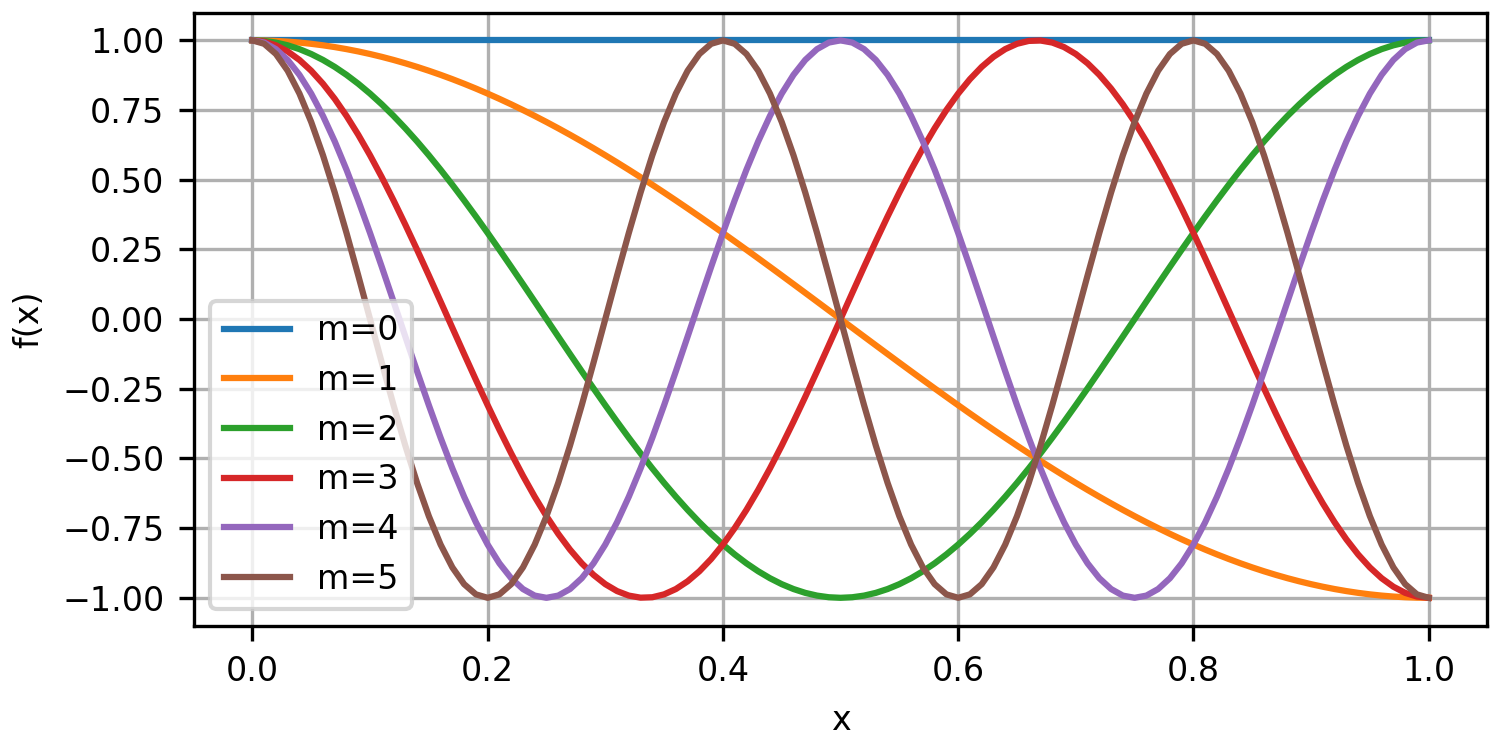
\includegraphics[width=5in]{1bfig1.png}
    \caption{$f(x) = \sin(\pi m x)$ for $\mathrm{d}x=0.01$ and $m=\{0, 1, 2, 3, 4, 5\}$}
    \label{1bfig1}
\end{figure}

\begin{listing}[H]
    \caption{Python code to compute inner products}
    \label{1blst2}
    \begin{minted}{python}
        mn_pairs = [(1, 4), (2, 6), (3, 15)]
        for m, n in mn_pairs:
            x = np.arange(0, 1.01, 0.01)
            f = np.sin(m * np.pi * x)
            g = np.sin(n * np.pi * x)
            inner_prod = integrate.trapezoid(y=f*g, x=x)
            print(f"Inner product of m={m} and n={n} is: {inner_prod}")
    \end{minted}
    \begin{minted}{python-console}
        Inner product of m=1 and n=4 is: -1.0963994469259664e-17
        Inner product of m=2 and n=6 is: -1.3227266504323154e-17
        Inner product of m=3 and n=15 is: -2.439454888092385e-18
    \end{minted}
\end{listing}

%%%%%%%%%%%%%%%%%%%%%%%%%%%%%%%%%%%%%%%%%%%%%%%%%%%%%%%%%%%%%%%%%%%%%%%%%%%%%%%%
% 2. Inner Product, Revisited
%%%%%%%%%%%%%%%%%%%%%%%%%%%%%%%%%%%%%%%%%%%%%%%%%%%%%%%%%%%%%%%%%%%%%%%%%%%%%%%%
\section{Inner Product, Revisited}

\subsection{} % a --------------------------------------------------------------
Sine and cosine waves are orthogonal.
\begin{mdframed}
    $\langle a, b \rangle$ is zero
\end{mdframed}

\subsection{} % b --------------------------------------------------------------
Although dissimilar, the signals are in phase.
\begin{mdframed}
    $\langle b, c \rangle$ is close to one
\end{mdframed}

\subsection{} % c --------------------------------------------------------------
$a(x)$ is odd and $d(x)$ is even; they are orthogonal.
\begin{mdframed}
    $\langle a, d \rangle$ is zero
\end{mdframed}

\subsection{} % d --------------------------------------------------------------
$f(x)$ is a rescaled $a(x)$.
The inner product is just the product of the magnitudes.
\begin{mdframed}
    $\langle a, f \rangle$ is greater than one
\end{mdframed}

%%%%%%%%%%%%%%%%%%%%%%%%%%%%%%%%%%%%%%%%%%%%%%%%%%%%%%%%%%%%%%%%%%%%%%%%%%%%%%%%
% 3. Image Compression
%%%%%%%%%%%%%%%%%%%%%%%%%%%%%%%%%%%%%%%%%%%%%%%%%%%%%%%%%%%%%%%%%%%%%%%%%%%%%%%%
\section{Image Compression}

\setcounter{subsection}{1} % skip subsection 1
\subsection{} % b --------------------------------------------------------------
\begin{figure}[H]
    \centering
    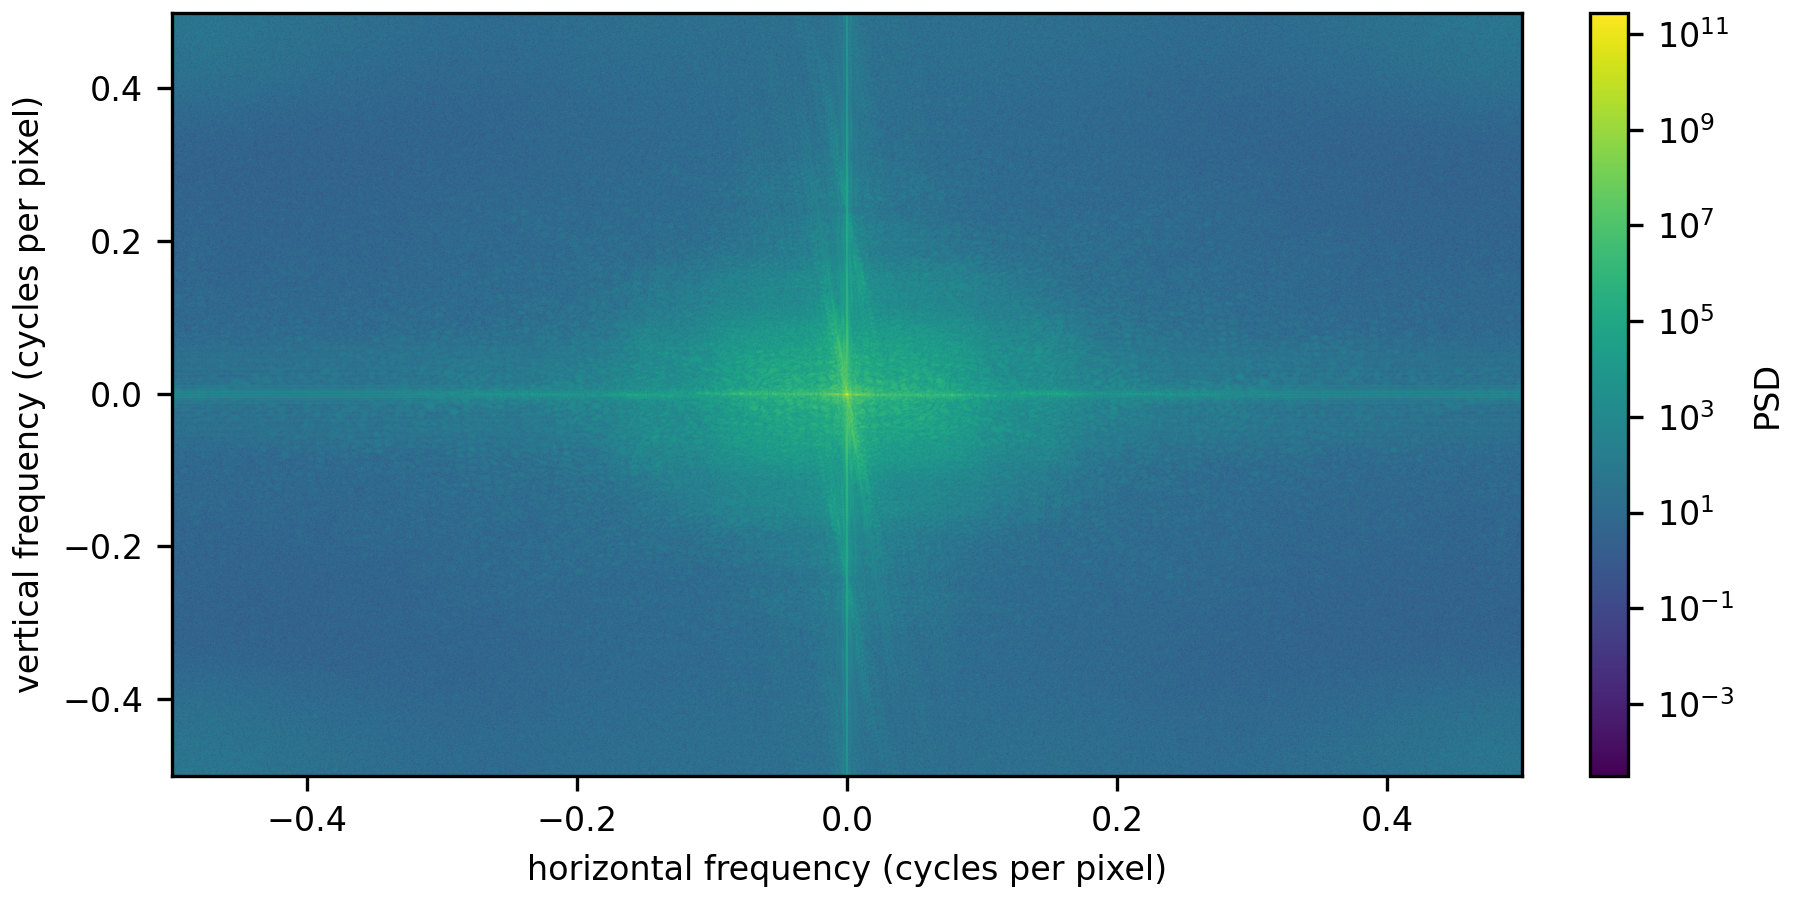
\includegraphics[width=6.5in]{3bfig1.png}
    \caption{Power spectral density of Fourier coefficients of image}
    \label{3bfig1}
\end{figure}

\subsection{} % c --------------------------------------------------------------
\begin{figure}[H]
    \centering
    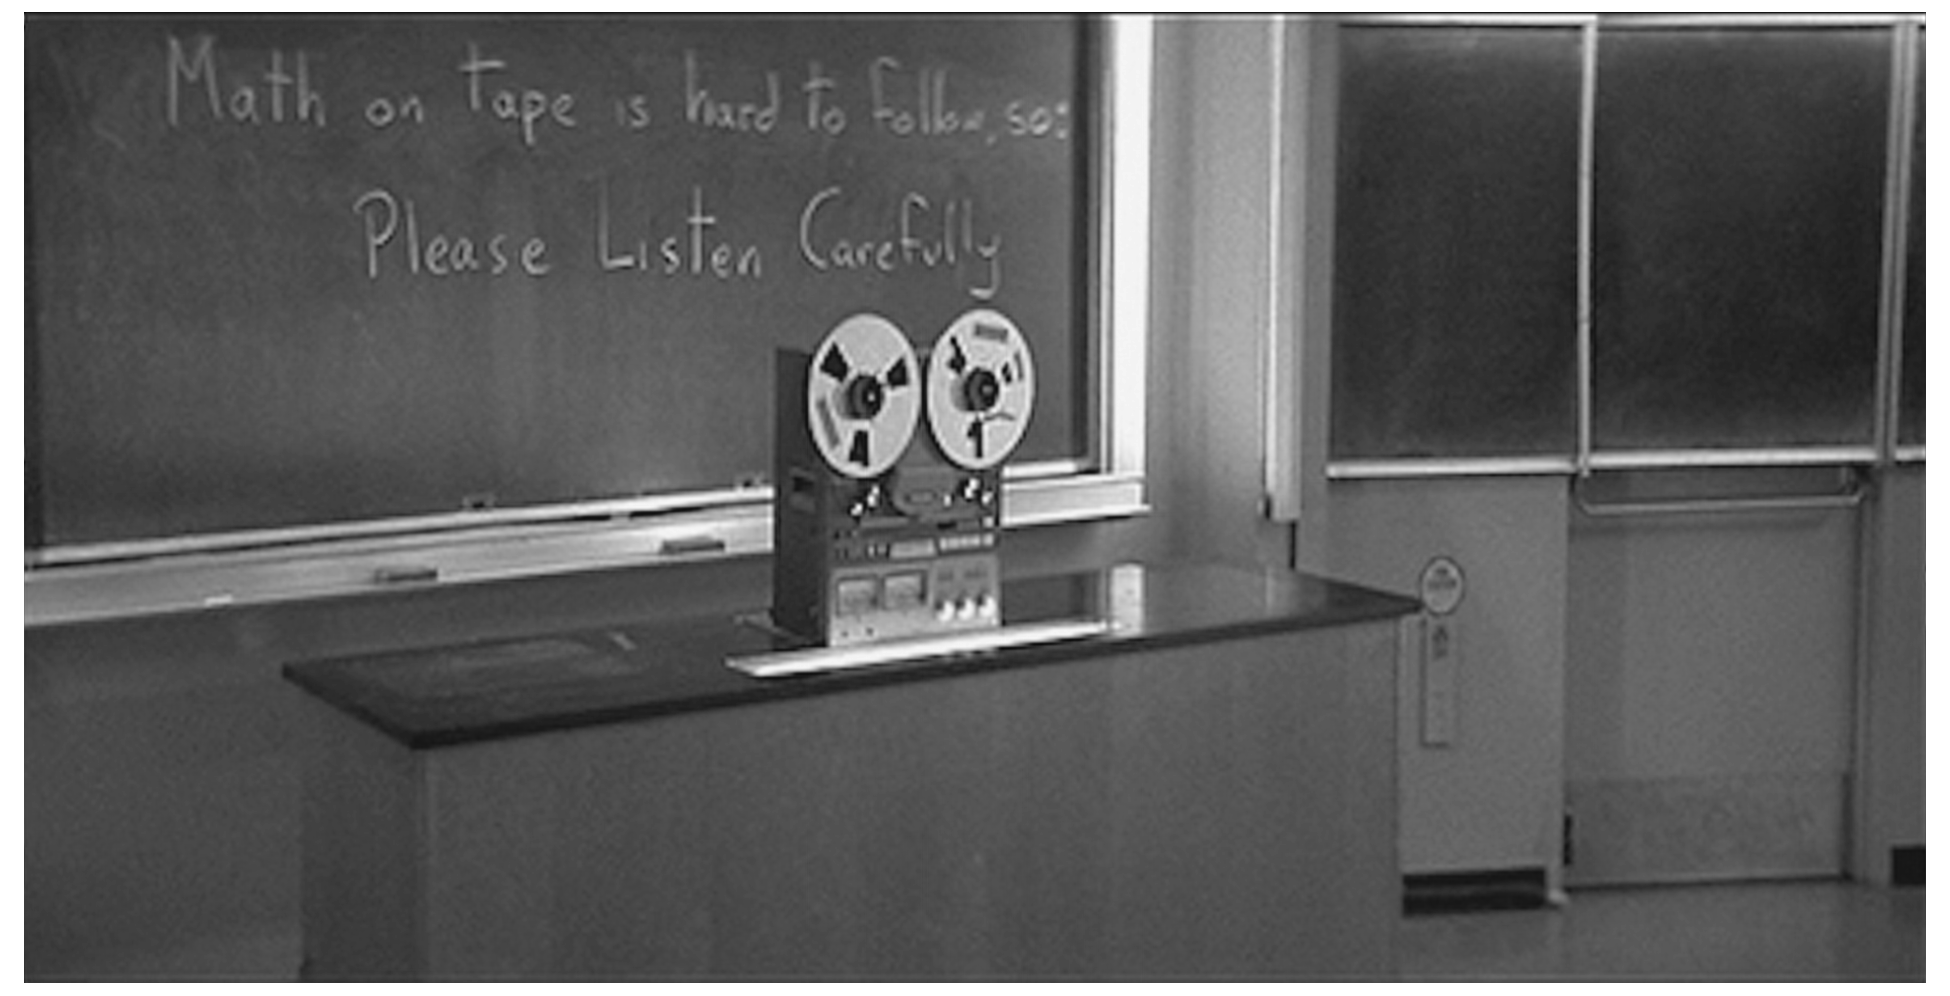
\includegraphics[width=6.5in]{3cfig1.png}
    \caption{Image with 10\% of original Fourier coefficients}
    \label{3cfig1}
\end{figure}
\begin{figure}[H]
    \centering
    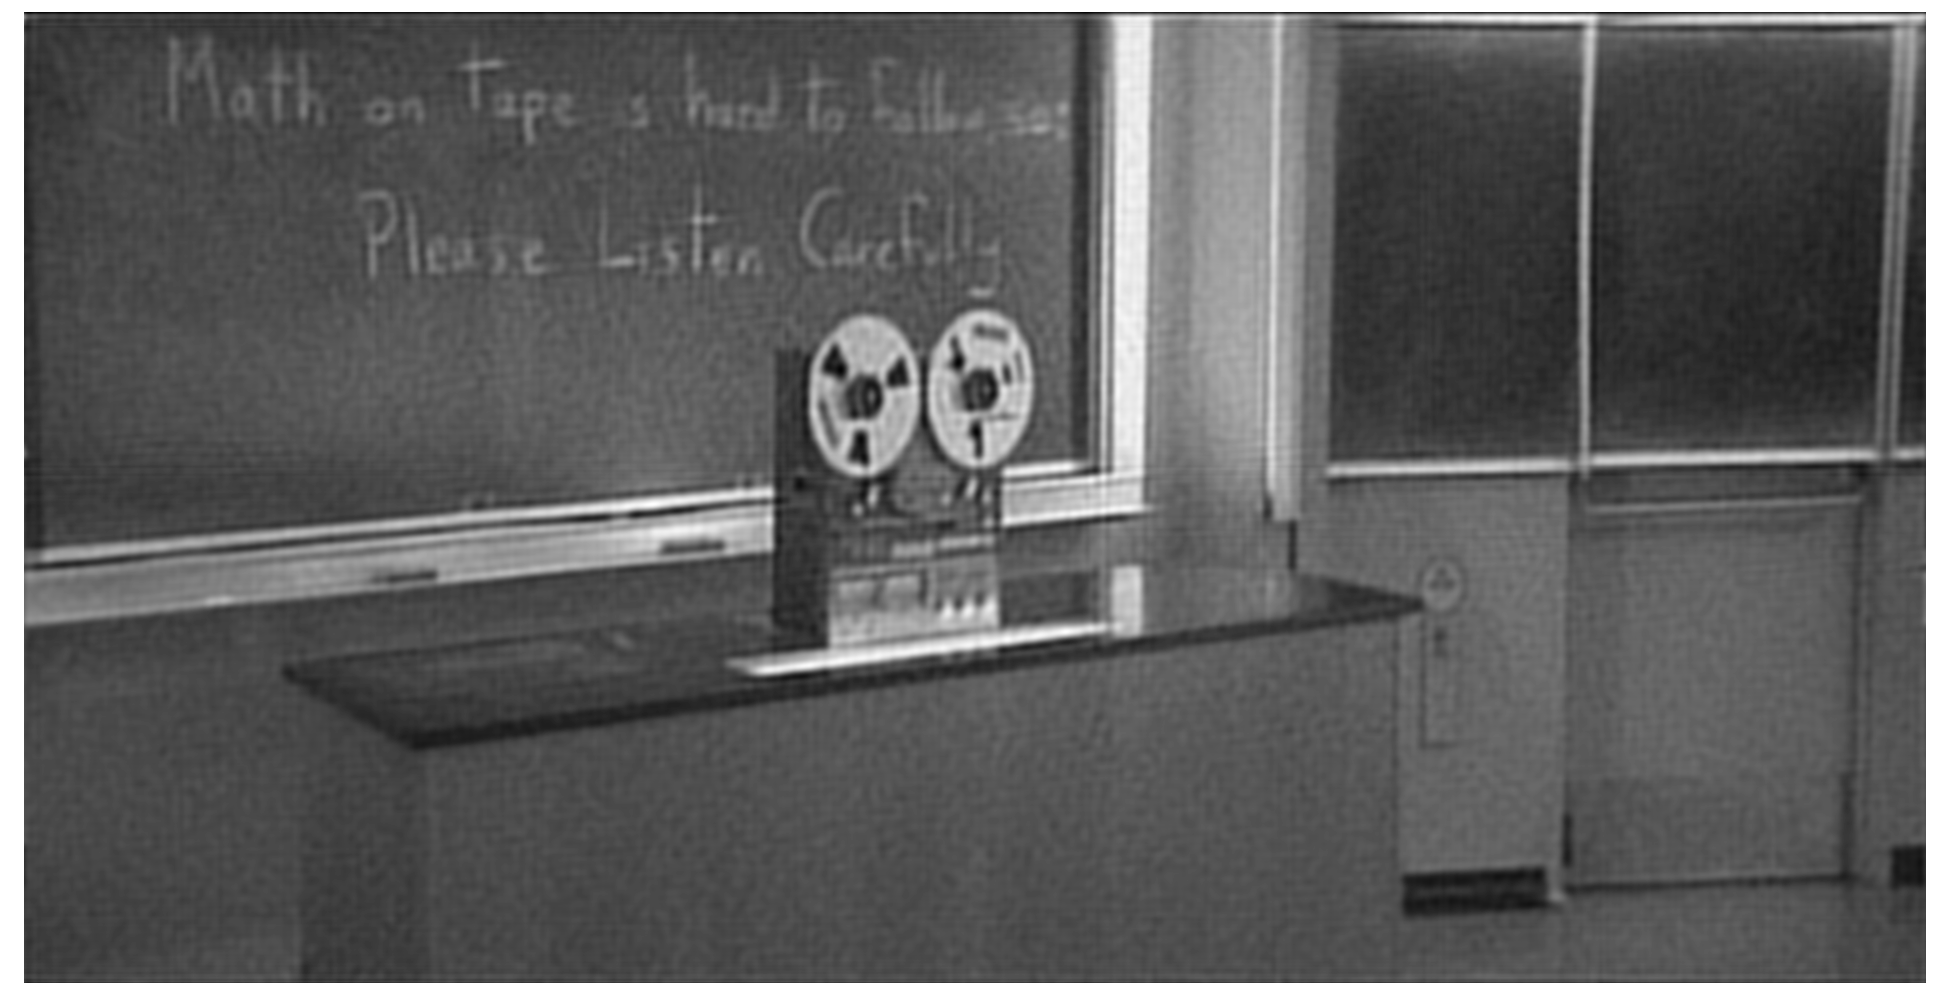
\includegraphics[width=6.5in]{3cfig2.png}
    \caption{Image with 1\% of original Fourier coefficients}
    \label{3cfig2}
\end{figure}
\begin{figure}[H]
    \centering
    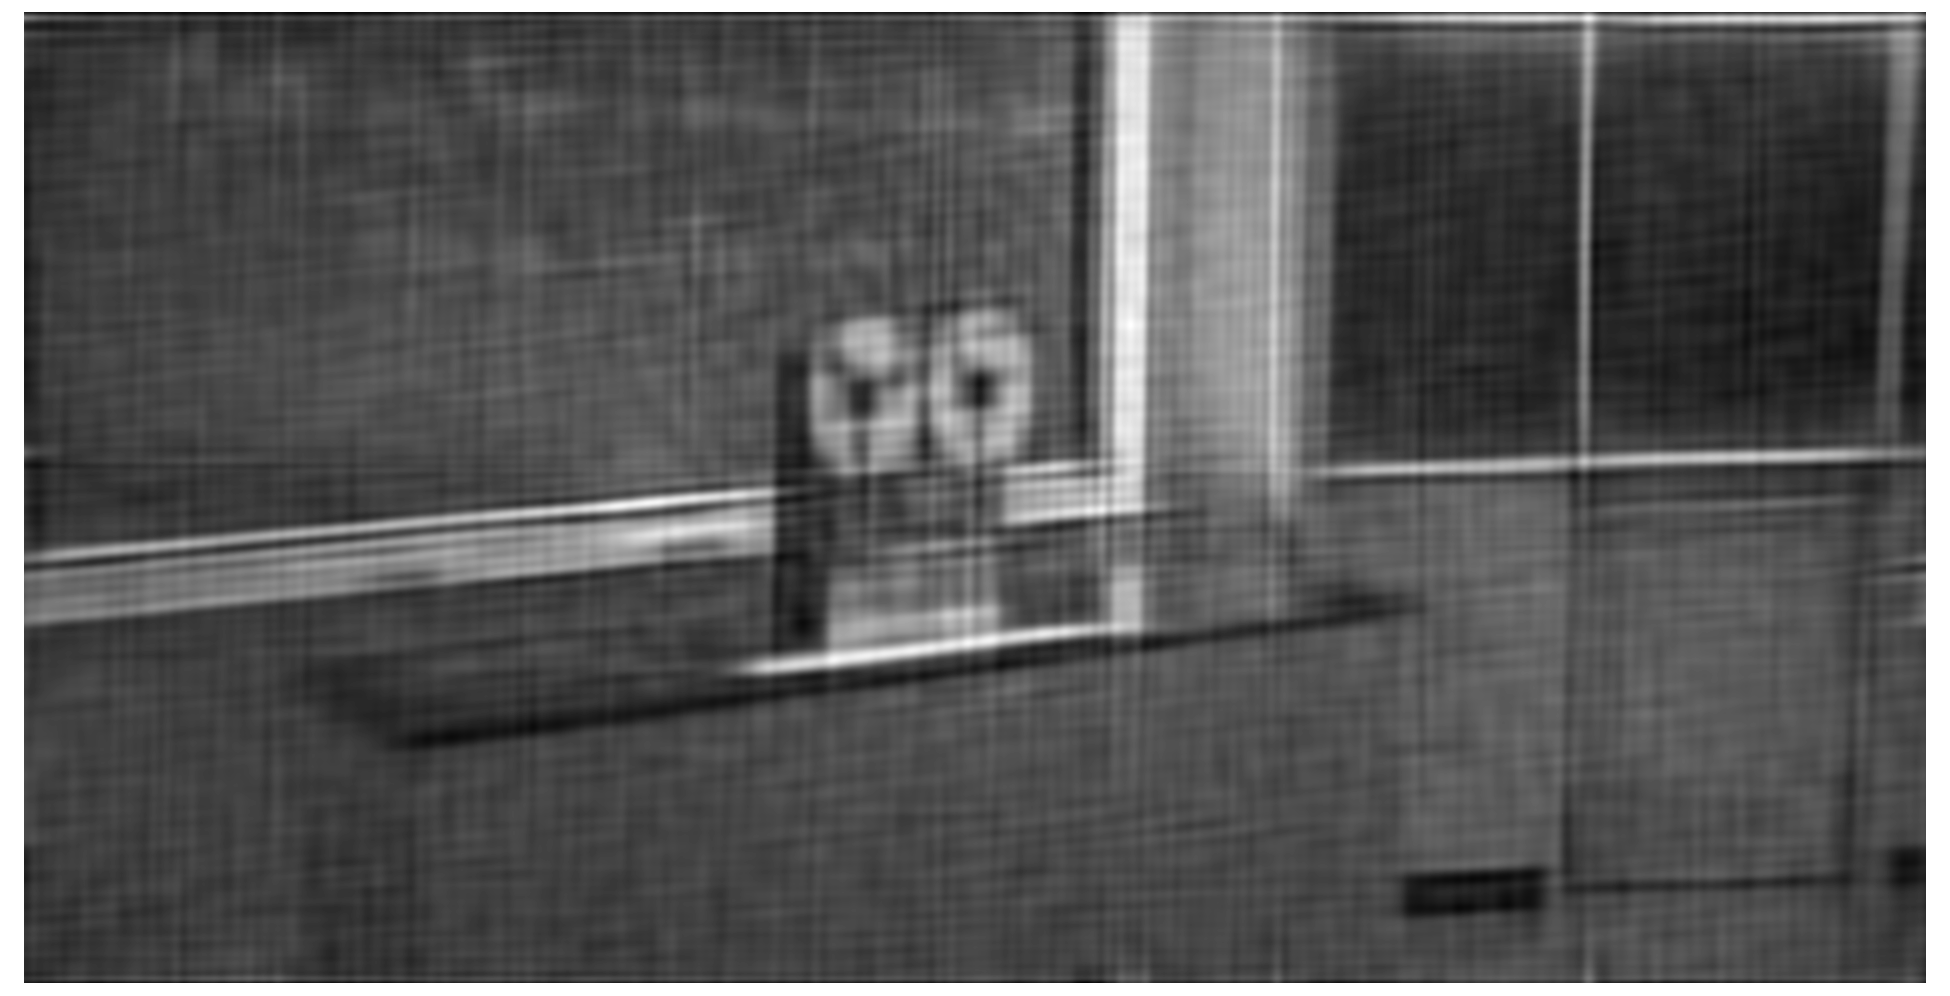
\includegraphics[width=6.5in]{3cfig3.png}
    \caption{Image with 0.2\% of original Fourier coefficients}
    \label{3cfig3}
\end{figure}

\subsection{} % d --------------------------------------------------------------
Keeping 10\% of the Fourier coefficients yields an image which is visually
indiscernible from the original because the magnitude of the truncated Fourier
coefficients is negligible.

Keeping 1\% of the Fourier coefficients yields an image which is visually
less detailed and more noisy than the original because the magnitude of the
truncated Fourier coefficients is significant.

Keeping 0.2\% of the Fourier coefficients yields an image which is lacking major
details/features because large Fourier coefficients have been truncated,
significantly altering the result. Stripe-like artifacts appear which result
from the interference patterns of the remaining low-frequency components.

\setcounter{subsection}{1} % skip subsection 5

%%%%%%%%%%%%%%%%%%%%%%%%%%%%%%%%%%%%%%%%%%%%%%%%%%%%%%%%%%%%%%%%%%%%%%%%%%%%%%%%
% 4. Fourier Series vs Fourier Transform
%%%%%%%%%%%%%%%%%%%%%%%%%%%%%%%%%%%%%%%%%%%%%%%%%%%%%%%%%%%%%%%%%%%%%%%%%%%%%%%%
\section{Fourier Series vs Fourier Transform}

\subsection{} % a --------------------------------------------------------------
The Fourier series representation of $f(x)$ on the interval with width $L=4$ is
\begin{align*}
    f(x) &= \frac{A_0}{2} + \sum_{k=1}^\infty \left[
        A_k \cos\left( \frac{2 \pi k}{L} x \right)
        + B_k \sin\left( \frac{2 \pi k}{L} x \right)
        \right]
\end{align*}
where $A_0$ is given by
\begin{align*}
    A_0 &= \frac{2}{L} \int_{L/2}^{L/2} f(x) \mathrm{d}x \\
    A_0 &= \frac{2}{4} \int_{-2}^{2} f(x) \mathrm{d}x \\
    A_0 &= \frac{1}{2} \left[
        \int_{-2}^{-1} 0 \mathrm{d}x
        + \int_{-1}^{1} 1 \mathrm{d}x
        + \int_{1}^{2} 0 \mathrm{d}x
        \right] \\
    A_0 &= 1
\end{align*}
and where $A_k$ is given by
\begin{align*}
    A_k &= \frac{2}{L} \int_{L/2}^{L/2} f(x) \cos\left(\frac{2 \pi k}{L}x\right) \mathrm{d}x \\
    A_k &= \frac{2}{4} \left[
        \int_{-2}^{-1} 0 \cdot \cos\left(\frac{2 \pi k}{4}x\right) \mathrm{d}x
        + \int_{-1}^{1} 1 \cdot \cos\left(\frac{2 \pi k}{4}x\right) \mathrm{d}x
        + \int_{1}^{2} 0 \cdot \cos\left(\frac{2 \pi k}{4}x\right) \mathrm{d}x
        \right] \\
    A_k &= \frac{1}{2} \int_{-1}^{1} \cos\left(\frac{\pi k}{2}x\right) \mathrm{d}x \\
    A_k &= \frac{1}{2} \left[ \frac{\sin\left(\frac{\pi k}{2} x\right)}{\pi k / 2} \right]_{-1}^{1} \\
    A_k &= \frac{1}{\pi k} \left[ \sin\left(\frac{\pi k}{2}\right) - \sin\left(-\frac{\pi k}{2}\right) \right] \\
    A_k &= \frac{1}{\pi k} \left[ \sin\left(\frac{\pi k}{2}\right) + \sin\left(\frac{\pi k}{2}\right) \right] \\
    A_k &= \frac{2}{\pi k} \sin\left(\frac{\pi k}{2}\right)
\end{align*}
and where $B_k$ is given by
\begin{align*}
    B_k &= \frac{2}{L} \int_{L/2}^{L/2} f(x) \sin\left(\frac{2 \pi k}{T}x\right) \mathrm{d}x \\
    B_k &= 0
\end{align*}
since $f(x) \cdot \sin\left(\frac{2 \pi k}{T}x\right)$ is an odd function.

Thus, the Fourier series representation of $f(x)$ on the interval $[-2, 2]$ is
\begin{align*}
    \Aboxed{
        f(x) &= \frac{1}{2} + \sum_{k=1}^\infty
        \frac{2}{\pi k} \sin\left(\frac{\pi k}{2}\right)
        \cos\left( \frac{\pi k}{2} x \right)
    }
\end{align*}
% Since $\sin\left(\frac{\pi k}{2}\right)$ is one for odd values of $k$ and zero otherwise,
% the terms with even-valued $k$ can be dropped.
% \begin{align*}
%     \Aboxed{
%         f(x) &= \frac{1}{2} + \sum_{k=1}^\infty
%         \frac{2}{\pi (2k-1)} (-1)^{k-1}
%         \cos\left( \frac{\pi (2k-1)}{2} x \right)
%     }
% \end{align*}

\subsection{} % b --------------------------------------------------------------
\begin{listing}[H]
    \caption{Python code to generate Figure \ref{4bfig1}}
    \label{4blst1}
    \begin{minted}{python}
        # Compute fourier series mode coefficients
        k = np.arange(1, 101)
        Ak = 2/(np.pi*k)*np.sin(np.pi*k/2)
        Bk = k*0

        # Plot fourier series mode coefficients
        fig, ax = plt.subplots(figsize=(6.5, 3.5), layout='constrained')
        ax.plot(k, Ak, '.', label='$A_k$')
        ax.plot(k, Bk, '+', label='$B_k$')
        ax.set_xlabel('$k$')
        ax.set_ylabel('Mode coefficient')
        ax.legend()
        ax.grid(True)
        fig.savefig('4bfig1.png', dpi=300)
        plt.show()
    \end{minted}
\end{listing}

\begin{figure}[H]
    \centering
    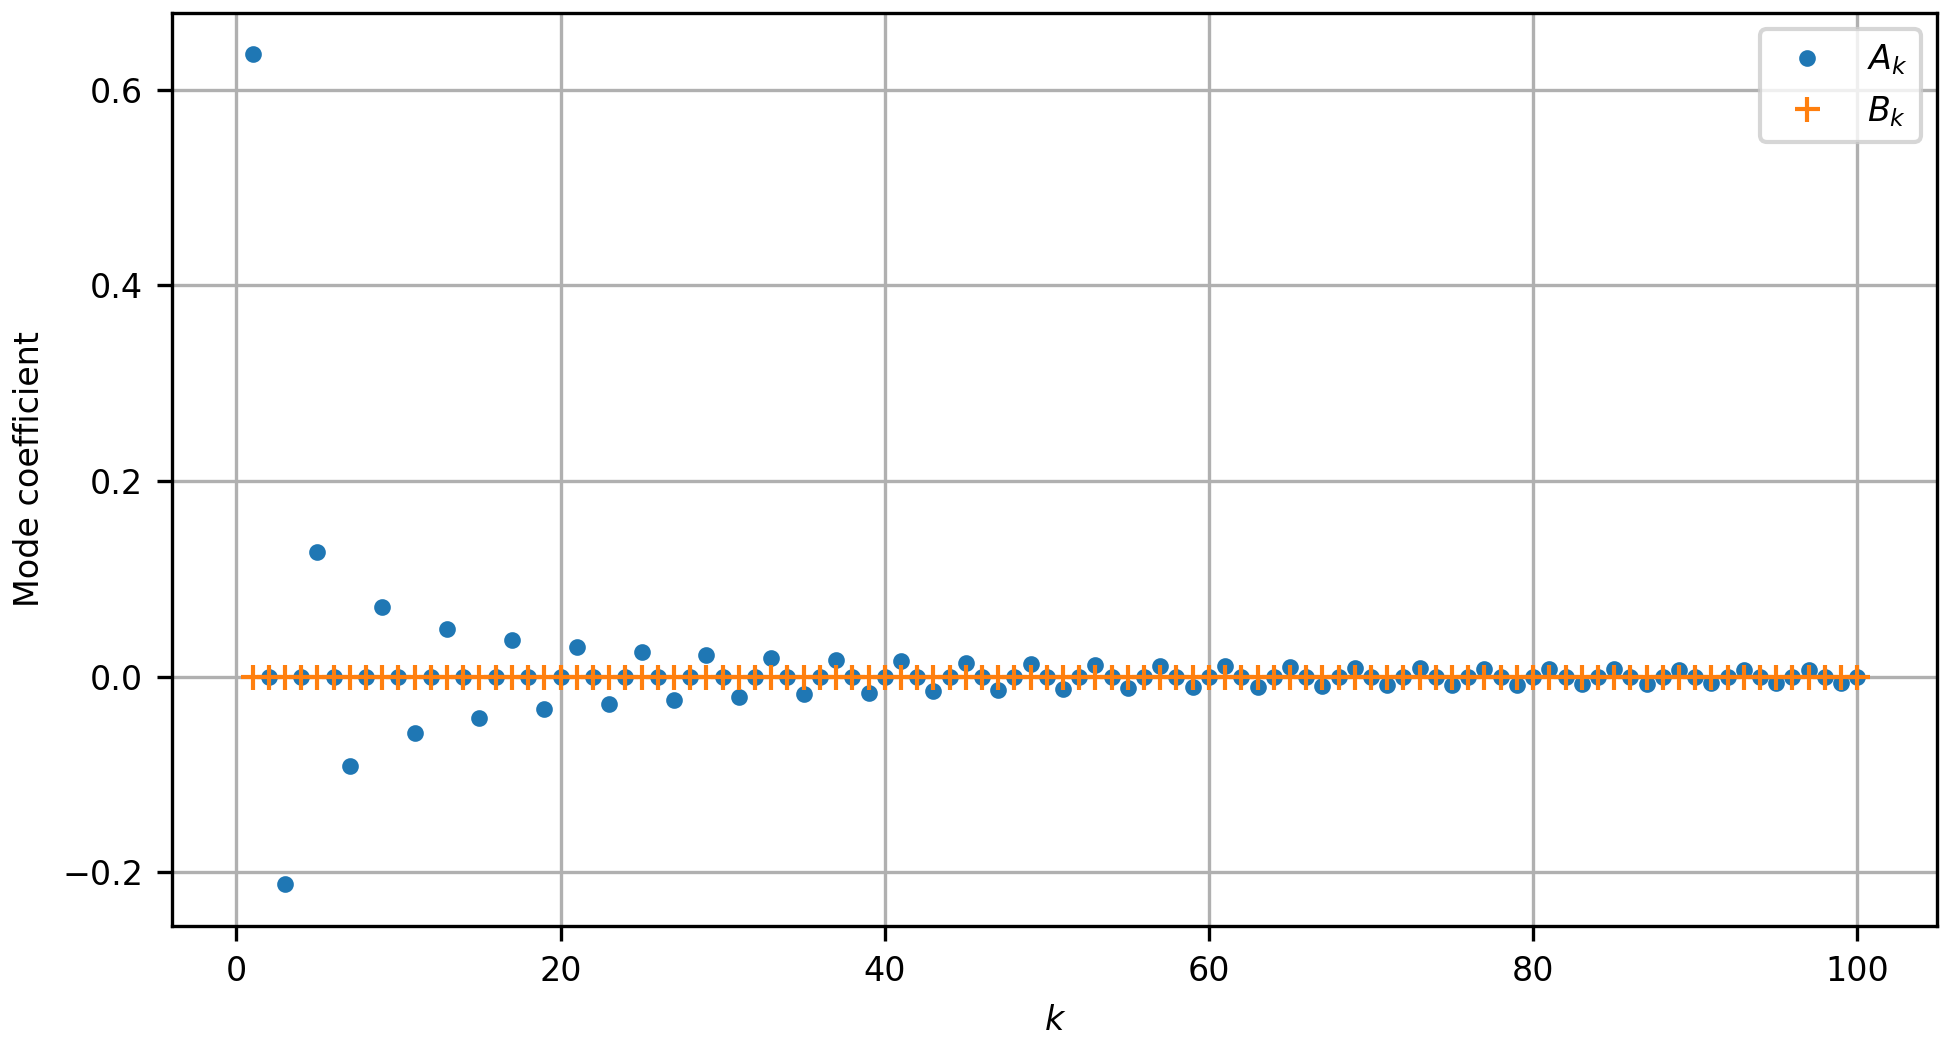
\includegraphics[width=6.5in]{4bfig1.png}
    \caption{Fourier series mode coefficients of $f(x)$}
    \label{4bfig1}
\end{figure}

\subsection{} % c --------------------------------------------------------------
\begin{listing}[H]
    \caption{Python code to generate Figure \ref{4cfig1}}
    \label{4clst1}
    \begin{minted}{python}
    # Define square wave function
        def square(x):
            return np.mod(x-1, 4) >= 2

        # Define fourier series square wave approximation function
        def square_approx(x, n):
            sum = 0.5 + np.zeros(x.shape)
            for k in range(1, n+1):
                sum += 2/(np.pi*k) * np.sin(np.pi*k/2) * np.cos(np.pi*k/2*x)
            return sum

        # Plot square wave function
        dx = 0.01
        x_vec = np.arange(-2, 2+dx, dx)

        fig, ax = plt.subplots(figsize=(5, 3), layout='constrained')
        ax.plot(x_vec, square(x_vec), 'k--', label='truth')
        ax.plot(x_vec, square_approx(x_vec, 10), label='Fourier series approx.')
        ax.set_xlabel('$x$')
        ax.set_ylabel('$f(x)$')
        ax.legend()
        fig.savefig('4cfig1.png', dpi=300)
        plt.show()
    \end{minted}
\end{listing}

\begin{figure}[H]
    \centering
    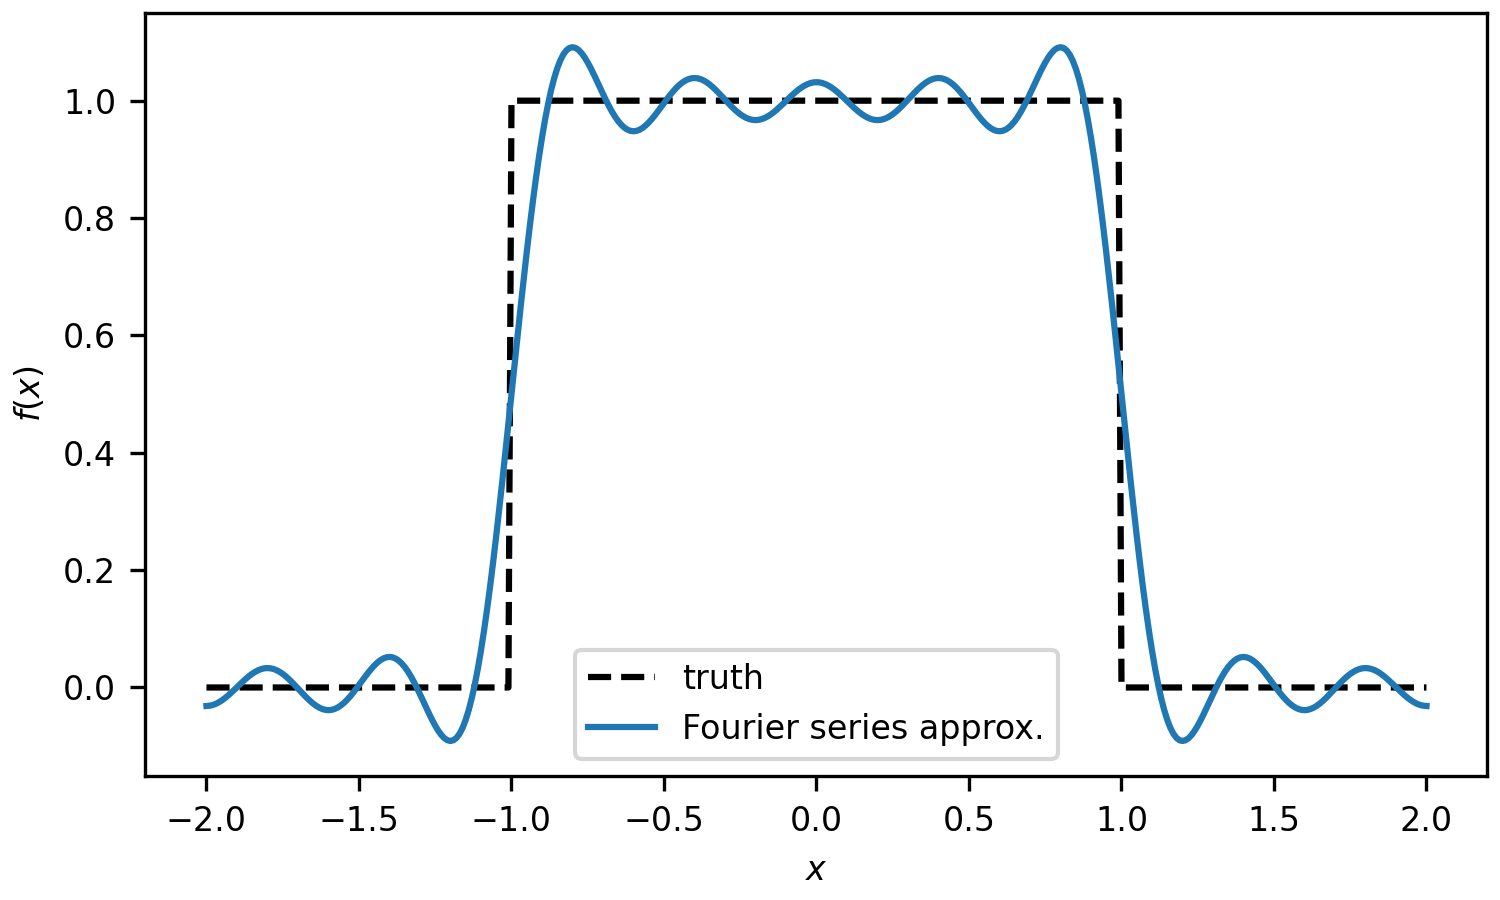
\includegraphics[width=5in]{4cfig1.png}
    \caption{$k=10$ Fourier series approximation of $f(x)$}
    \label{4cfig1}
\end{figure}

\subsection{} % d --------------------------------------------------------------
Assuming that $f(x)$ is zero for all $x<-1$ and $x>1$,
\begin{align*}
    \mathcal{F}(f(x)) &= \fourier{f(x)} \\
    \mathcal{F}(f(x)) &=
        \int_{-\infty}^{-1} 0 \cdot e^{i \omega x} \mathrm{d}x
        +\int_{-1}^{1} 1 \cdot e^{i \omega x} \mathrm{d}x
        + \int_{1}^{\infty} 0 \cdot e^{i \omega x} \mathrm{d}x \\
    \mathcal{F}(f(x)) &= \int_{-1}^{1} e^{i \omega x} \mathrm{d}x \\
    \mathcal{F}(f(x)) &= \left[ \frac{e^{i \omega x}}{i \omega} \right]_{-1}^{1} \\
    \Aboxed{
        \mathcal{F}(f(x)) &= \frac{e^{i \omega} - e^{-i \omega}}{i \omega}
        }
\end{align*}

\subsection{} % e --------------------------------------------------------------
\begin{mdframed}
    The Fourier series is a representation of a periodic function $f$ with
    period $T$ in a new discrete basis. The basis is discrete because only
    functions which have periods $T_k$ which are integer fractions of $T$ are
    valid basis functions. The Fourier transform extends this to non-periodic
    (or infinite-period) functions $f$. A consequence of this is that all
    frequencies of basis function are valid, so the basis is now continuous.
\end{mdframed}

%%%%%%%%%%%%%%%%%%%%%%%%%%%%%%%%%%%%%%%%%%%%%%%%%%%%%%%%%%%%%%%%%%%%%%%%%%%%%%%%
% 5. Using Spectrograms for Species ID
%%%%%%%%%%%%%%%%%%%%%%%%%%%%%%%%%%%%%%%%%%%%%%%%%%%%%%%%%%%%%%%%%%%%%%%%%%%%%%%%
\section{Using Spectrograms for Species ID}

\subsection{} % a --------------------------------------------------------------
\begin{mdframed}
    Sound features in the time-domain signal are spread across thousands of
    pressure samples, obscuring them from discovery and interpretation. In
    contrast, the spectrogram is a natural representation of the coherent
    features which differentiate sounds (including bird vocalizations).
    Spectrograms also naturally lend themselves as inputs to machine powerful
    learning architectures built for image classification.
\end{mdframed}

\subsection{} % b --------------------------------------------------------------
\begin{mdframed}
    The horizontal axis of a spectrogram is time (seconds) and the vertical axis
    of a spectrogram is frequency (Hz).
\end{mdframed}

\subsection{} % c --------------------------------------------------------------
\begin{mdframed}
    There is a direct trade-off between temporal resolution and frequency
    resolution in a spectrogram which is set by the window length. If a bird
    vocalization contained short-time features and broad frequencies, increasing
    the temporal resolution to capture the short-time features would degrade the
    ability to capture the extreme frequencies and vice versa. In this case,
    higher resolution source (time-domain) data must be obtained to capture the
    full range of features.
\end{mdframed}

\subsection{} % d --------------------------------------------------------------
\begin{mdframed}
    The fast Fourier transform's bisection algorithm requires data which has
    length equal to a power of 2.
\end{mdframed}

\subsection{} % e --------------------------------------------------------------
\begin{mdframed}
    The short-time Fourier transform (STFT) is a way to get a time-varying
    Fourier transform of a signal by breaking the signal into short "windows,"
    performing the Fourier transform on each window, and then joining the
    results to form a  two-dimensional time-frequency output. The temporal
    resolution is determined by the width of the windows, so shorter windows
    are required to attain fine temporal resolution. However, the discrete
    Fourier transform's frequency resolution is determined by the inverse of the
    width of the window, so wider windows are required to attain fine frequcy
    resolution.
\end{mdframed}

\subsection{} % f --------------------------------------------------------------
\begin{mdframed}
    The data varies in amplitude. Amplitude is mostly dependent on factors other
    than the features of the bird vocalization (e.g. distance from microphone,
    microphone sensitivity). Thus, normalization helps eliminate these unwanted
    variables.
\end{mdframed}

\subsection{} % g --------------------------------------------------------------
\begin{mdframed}
    Logarithmic scaling makes low-amplitude and high-amplitude features
    simultaneously interpretable.
\end{mdframed}

\subsection{} % h --------------------------------------------------------------
\begin{mdframed}
    They normalized the data with three unique methods and encoded each into a
    color channel. This allowed the machine learning model to utilize features
    that are made apparent using any of the three normalization methods.    
\end{mdframed}

\subsection{} % i --------------------------------------------------------------
\begin{mdframed}
    Deviating from logarithmic scaling can have potential for minor improvements
    in model accuracy but come with a large increase in computational cost.
\end{mdframed}

%%%%%%%%%%%%%%%%%%%%%%%%%%%%%%%%%%%%%%%%%%%%%%%%%%%%%%%%%%%%%%%%%%%%%%%%%%%%%%%%
% 5. Connections to Your Own Work
%%%%%%%%%%%%%%%%%%%%%%%%%%%%%%%%%%%%%%%%%%%%%%%%%%%%%%%%%%%%%%%%%%%%%%%%%%%%%%%%
\section{Connections to Your Own Work}

\subsection{} % a --------------------------------------------------------------
\begin{mdframed}
    High-frequency surface-mounted pressure sensors are used in wind tunnel
    tests to detect buffet onset and other aerodynamic features. Classification
    models could be trained to recognize buffet onset, transition to turbulence,
    and flow separation based on real-time surface pressure data in the
    frequency domain.
\end{mdframed}

\subsection{} % b --------------------------------------------------------------
\begin{mdframed}
    I would use a spectrogram. The system is time-varying as the model
    pitches/yaws in the wind tunnel, so the FFT is inappropriate. Since the data
    is extremely noisy and high-frequency, a frequency-domain approach would be
    required to isolate the coherent features.
\end{mdframed}

\end{document}